\subsubsection{退化初级场与平凡单值性}\label{degtriv}


现在我们来回顾关于 Virasoro 代数表示的一些标准事实。这将使我们能够说明，由自由场表示得到的那些特定共形块究竟特殊在哪里。


对于一般的共形维数 $\Delta$，由维数为 $\Delta$ 的最高权向量的所有 Virasoro 后代张成的 Verma 模是不可约的。但对一组特殊值
\begin{equation} \alpha = \alpha_{r,s} = - \frac{(r-1) b}{2} - \frac{s-1}{2 b},~~~r,s=1,2,3,\dots \end{equation}
或 $\alpha = Q- \alpha_{r,s}$，情况并非如此：某一层数为 $r s$ 的后代再次成为最高权向量，并且具有零模。在幺正的共形场论中，该后代将会消失；即便在非幺正的理论中，它也可能消失。后代消失的初级场称为退化初级场。我们把这样的场记作 $\Phi_{r,s}$。
% [Tutor Note: 约定差异] 注意 $\Delta=\alpha(Q-\alpha)$ 在 $\alpha\leftrightarrow Q-\alpha$ 下不变，所以退化值总成对出现：$\alpha_{r,s}$ 与 $Q-\alpha_{r,s}$ 给出同一个共形维数，而 $r\leftrightarrow s$ 一般给出不同的值。引用退化值时不要漏掉 $Q-\alpha_{r,s}$ 这一支。


退化初级场的消失后代在关联函数中当然会退耦。我们把满足这种关系的共形块称为退化共形块。它们满足一个称为“退化融合规则”的条件。（这可以用我们马上要提到的微分方程来证明。）在算符 $\Phi_{r,s}$ 与动量为 $\alpha$ 的算符的 OPE 中，只出现动量为 $\alpha - \frac{r' b}{2} - \frac{s'}{2 b}$ 的算符，其中
\begin{equation}
r' = r-1 , r-3, \cdots ,1-r \qquad s' = s-1, s-2 \cdots ,1-s.
\end{equation}

插入动量为 $\alpha_{r,s}$ 的共形块满足零态退耦条件，当且仅当其关联函数满足某个 $rs$ 阶微分方程。一个重要的特例是 $r=2$、$s=1$；此时方程为
\begin{equation}\label{opeq2}
\partial^2 \Phi_{2,1}(z) + b^2 : T(z) \Phi_{2,1}(z): =0.
\end{equation}
% [Tutor Note: 易错点] (\ref{opeq2}) 中的系数是 $b^2$ 而不是 $b^{-2}$：$b\to0$ 时左边第二项就是 $b^2T\to\bt$，于是 (\ref{opeq2}) 化为 (\ref{opeq}) 的 $\partial^2 f+\bt f=0$。（$\Phi_{2,1}$ 的动量 $\alpha=-b/2$ 给出维数 $\Delta=1-\frac{3}{4}b^2\to1$ 的“轻”场，与 $V_{-k/2b}$ 那类“重”场不同。）此处 $T$ 的归一化与 (\ref{opeq2}) 的写法一致，换约定时符号/系数会变，核对时以原文为准。

这半经典极限下化为与 oper 相联系的微分方程 (\ref{opeq})。（当 $b\to 0$ 时，(\ref{opeq2}) 中的正规序无关紧要；$b^2T$ 中在 $b\to 0$ 时存活下来的部分，只是对动量为 $1/b$ 量级的“重”场的响应。）此外，在半经典极限下，$\bt=b^2T$ 的期望值总是使得微分方程绕带有额外 $\Phi_{1,s}$ 插入的点一周的单值性为平凡。事实上，退化融合规则蕴含 $\Phi_{2,1}$ 与 $\Phi_{1,s}$ 的 OPE 只包含一个初级场 $\Phi_{2,s}$；由此可知，$\Phi_{2,1}$ 绕 $\Phi_{1,s}$ 穿刺点的单值性为平凡。这是与 oper 相联系的微分方程 (\ref{opeq}) 上平凡单值性条件的量子版本。另一方面，$\bt$ 在 $\Phi_{1,s}$ 插入点附近的奇点，正是我们在 (\ref{roog}) 中所展现的那种（其中 $j=s/2$）。由此得到的结论是：关联函数 $\left\langle \prod_{a=1}^d\Phi_{1,k_a}(z_a)\right\rangle$ 的共形块的半经典极限，确定了一个具有我们在第~\ref{opsing}~节中从三维规范场论提取出的那种无单值性奇点的 oper。
% [Tutor Note: 指标提醒] 按上述 $\alpha_{r,s}$ 公式，$\Phi_{1,s}$ 的动量是 $-\frac{s-1}{2b}$；而文中把它的极点与 $j=s/2$ 匹配（并与前文 $\alpha_a=-k_a/2b$ 的“重”场对应）。两者相差 $1/2b$，是 $\Phi_{1,s}$ 的标号与 $\alpha_{r,s}$ 标号之间的偏移；阅读时请以极点阶数 $j$（即 (\ref{roog}) 的系数）为准，不要直接把 $s=k_a$ 代进 $\alpha_{r,s}$。

由自由场公式 (\ref{freeinto}) 构造的共形块描述退化初级场的关联函数，这仅仅是因为动量为 $-\frac{k_a}{2b}$ 的自由场顶点算符是退化的。与此相关，可以证明由自由场实现给出的共形块确实满足退化融合约束。相应的微分方程等价于自由场积分所满足的 Picard-Fuchs 方程，或等价于积分链空间上的自然平坦联络。它们与 Knizhnik-Zamolodchikov 方程非常类似。自由场实现给出了关联函数 $\left\langle \prod_{a=1}^d\Phi_{1,k_a}(z_a)\right\rangle$ 在融合规则允许范围内的全部共形块，此外不再有别的共形块。

用退化共形场的关联函数来解释具有无单值性奇点的 oper，为 Bethe 方程提供了一个直观的解释。自然地，$\bt$ 在点 $w_i$ 处不应有极点，因为那里没有插入任何共形场。


\section{四维解与平行移动}\label{fourd}
\begin{keytakeaways}
\begin{itemize}\setlength{\itemsep}{2pt}
  \item \textbf{物理图像}：四维 BPS 方程的解可按“梯度流 + 针（thimble）”来理解——时间无关的经典解是 Morse 函数 $h=\mathrm{Re}(e^{i\alpha}\W)$ 的临界点，瞬子则是连接临界点的梯度流线；由于 $h$ 是全纯函数的实部，各临界点具有相同的中间维 Morse 指标，故瞬子不会抬升真空简并性。
  \item \textbf{数学工具}：无穷维 Morse 理论、相对同调 $H(\U,\U_<)$、Lefschetz 针、Stokes 墙，以及相对同调上的 Gauss-Manin 联络；量子基态与针一一对应，$\hat\H$ 因而带有整结构与自然的平坦联络。
  \item \textbf{主要结论}：纽结位置随时间缓慢变化时，基态的演化只通过穿过 Stokes 墙时的 Stokes 因子体现，传输矩阵元可由“混合路径”计数得到；且时间依赖情形的解数 $\frak N^J_I$ 等于仅由时间无关问题算出的 $\frak n^J_I$。
  \item \textbf{对偶基}：向上流的针 $\K^I$ 构成 Poincaré 对偶的相对同调 $H(\U,\U_>)$ 的基，配对 $\langle\K^J,\J_I\rangle=\delta^J{}_I$ 把任一链 $\Gamma$ 展开为针的线性组合。
\end{itemize}
\end{keytakeaways}
\subsection{引言}\label{fourdintro}

现在我们转向分析原始 BPS 方程 (\ref{bpseqns}) 的依赖时间的解。尽管这是一个经典偏微分方程的问题，量子力学的视角仍然是有益的。

\begin{figure}
 \begin{center}
     % >>> 原文图 6（原稿第 45 页）
  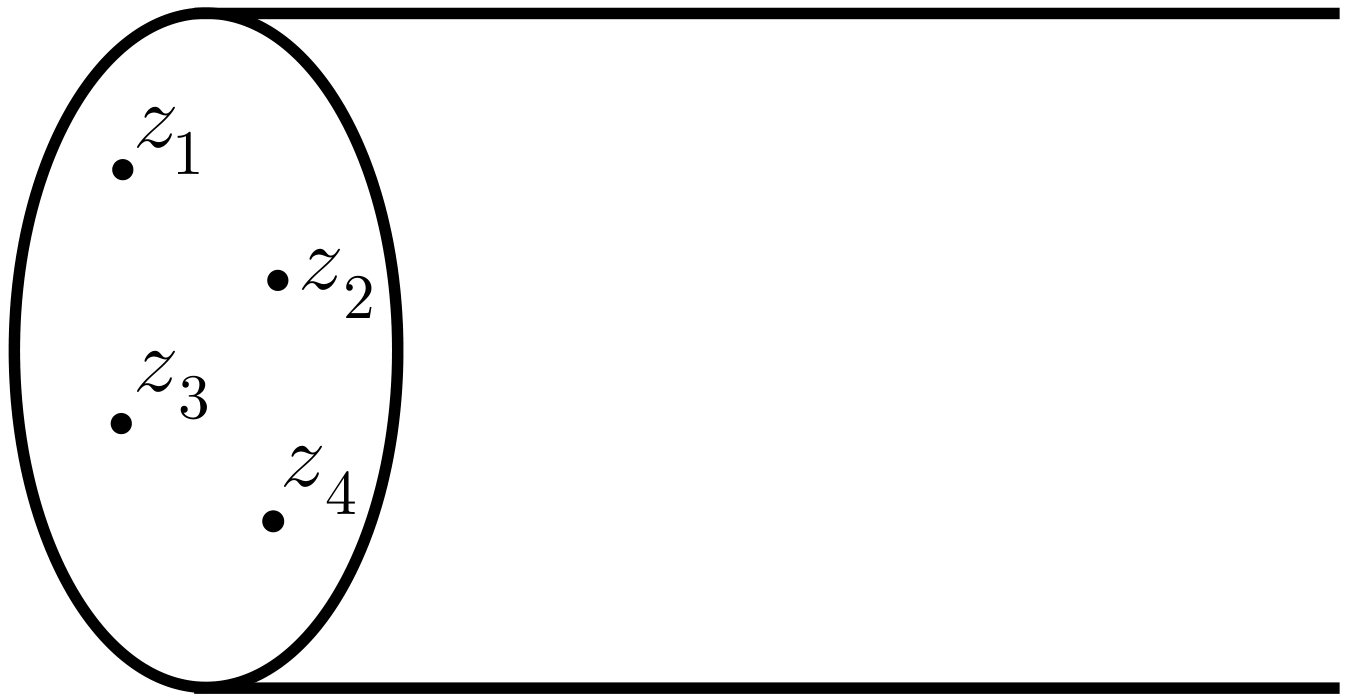
\includegraphics[width=3.5in]{figs/Fig06.png}
 \end{center}
\caption{\small  一个与时间无关的情形在固定时刻的快照。在三流形 $M_3=C\times \R_+$ 中，纽结出现在边界点 $z_1,\dots,z_4$ 处。（原稿第 45 页）}
 \label{again}
\end{figure}
我们从与时间无关的情形开始——四流形 $\MM=\R\times \Mthree$ 上的扭曲 $\N=4$ 超 Yang-Mills 理论，其中 $\Mthree$ 是一个三流形，而我们把 $\R$ 看作时间方向。在我们的应用中，$\Mthree=C\times \R_+$，$C$ 是黎曼面。若存在纽结，我们一开始假设它们与时间无关。在这种情形下（为方便起见，图~\ref{again} 再次描绘了它），我们要找出 BPS 态——量子基态。

第一步近似——已在第~\ref{teqone}~节与第~\ref{analog}~节中分析过——是寻找与时间无关的经典解。从经典解过渡到 BPS 态时，我们将忽略 $\Mthree$ 的非紧性。这意味着我们将忽略非 BPS 激发的连续谱的存在。


 若 BPS 方程只有有限多个经典解（且它们非退化——即围绕这样的解展开时没有零模），则 BPS 态空间的经典近似非常简单。令 $\I$ 为经典解的集合。于是对每个 $I\in \I$，微扰论中存在一个定域在 $I$ 附近的量子基态 $\psi_I$。在微扰论中，$\psi_I$ 构成 BPS 态空间 $\H$ 的一组基。

非微扰地看，在这类一般问题中，瞬子效应可能把这些近似基态中的一些从零能处抬升。然而，我们这里处理的实际上是不会发生这种情况的问题。这是因为在与时间无关的情形下，即便存在纽结，我们的问题也有四个超荷，而一个瞬子（即具有非平凡时间依赖性的经典解）至少破坏其中两个。这导致瞬子背景中出现两个费米零模，这比在近似基态 $\psi_I$ 与 $\psi_J$ 之间为超荷 $Q$ 的矩阵元作贡献所需的零模数多了一个。

\subsubsection{与 Morse 理论的关系}\label{relm}

关于瞬子为何不抬升经典真空简并性，一个更明确的理解来自于本问题与 Morse 理论的关系。\footnote{关于 Morse 理论相关方面相对易懂的介绍，见文献~\cite{hutchings}。}与 Morse 理论相关的超对称量子力学（文献~\cite{Morse}）一般是从 $\R$ 到 $\U$ 的映射的理论，其中 $\U$ 是带有度规张量 $g$ 的黎曼流形，并配有一个我们称为超势的实值函数 $h$。对一般的 $\U$ 与 $h$，该模型有两个超荷，其中一个与外微分共轭：
\begin{equation}\label{zolmo} Q=e^h\d e^{-h}.\end{equation}
经典真空对应于 $h$ 的临界点。若 $h$ 是 Morse 函数——即其临界点都是孤立且非退化的——则在微扰论中，每个临界点 $I$ 对应一个近似量子基态 $\psi_I$。$\psi_I$ 的费米子数 $q_I$ 等于临界点 $I$ 的 Morse 指标（即函数 $h$ 在 $I$ 处二阶导数矩阵的负本征值个数）。由于 $Q$ 使费米子数增加一个单位，只有当
\begin{equation}\label{yre} q_J=q_I+1.\end{equation}
时，才可能由量子修正诱导出非零矩阵元 $\langle \psi_J|Q|\psi_I\rangle$。这类非零矩阵元可以通过在适当意义下计数在远过去始于临界点 $I$、在远未来终于临界点 $J$ 的瞬子解来计算。相应的“瞬子”方程，换言之，映射 $\R\to \U$ 为 $Q$ 不变的条件，就是 Morse 理论的梯度流方程：
\begin{equation}\label{orlox} \frac{\d x^i}{\d t}=-g^{ij}\frac{\partial h}{\partial x^j}.\end{equation}

我们正在研究的 $\R\times \Mthree$ 上的扭曲 $\N=4$ 超 Yang-Mills 理论问题（我们主要取 $\Mthree=C\times\R_+$，但以下论述更为一般）就是这种类型的无穷维问题，\footnote{\label{zort}
更准确地说，我们的问题是这类问题的一个规范不变版本——对应于一个以 $\U$ 为目标、并与把 $\U$ 的一个对称性规范化的规范场耦合的超对称 sigma 模型。在我们的情形中，规范群是从 $\Mthree$ 到有限维群 $G$ 的映射构成的群，而 $\U$ 是 $\Mthree$ 上复值联络的空间。然而，在我们的问题中规范群自由地作用在 $\U$ 上；这由 Nahm 极点边界条件保证。因此，规范不变性不会起主要作用。实际上，就我们的目的而言，我们可以把 $\U$ 换作它对该复规范变换群的商，从而约化为没有规范场的情形。}其中 $\U$ 是 $\Mthree$ 上复值联络的空间。我们把 Chern-Simons 函数
\begin{equation}\label{csfun}\W=\frac{1}{4\pi i }\int_{\Mthree}\,\Tr\,\left(\A\wedge\d \A+\frac{2}{3}
\A\wedge\A\wedge\A\right)\end{equation}
看作复流形 $\U$ 上的全纯函数。全纯性意味着以 $\U$ 为目标、以 $\W$ 为超势的一维 sigma 模型有四个超荷（这实际上依赖于 $\U$ 的度规是 Kähler 度规这一事实，并且在脚注~\ref{zort} 提到的规范不变情形下也成立）。我们实际上希望在与 $\N=4$ 超 Yang-Mills 理论的某种扭曲相联系的框架中研究这个模型，其中某个特定的超荷 $Q$ 被专门标记出来。这个超荷依赖于扭曲参数 $\t$（文献~\cite{KW}），并且是 $Q=e^h\d e^{-h}$ 的无穷维版本，其中 $h$ 是通常的 Morse 函数
\begin{equation}\label{morsefn}h=\mathrm{Re}\,(e^{i\alpha}\W),\end{equation}
并且
\begin{equation}\label{alphaq} \t = \frac{1- \sin \alpha}{\cos{\alpha} }\end{equation}
对于这种类型的 Morse 函数，梯度流方程变为
\begin{equation}\label{lphaq} \frac{\d \bar w^{\bar j}}{\d t}=-g^{\bar j i}\frac{e^{i\alpha}}{2}
\frac{\partial\W}{\partial w^i},\end{equation}
其中 $w^i$ 是 $\U$ 上的局部全纯坐标。


我们的问题与 Morse 理论相联系的一个具体表现是：底层的四维超对称方程 (\ref{bpseqns}) 正是无穷维流形 $\U$ 上 Morse 函数 $h$ 的梯度流方程 (\ref{orlox})。（这是文献~\cite{Analytic,NewLook} 的主要思想之一，其中已把脚注~\ref{zort} 提到的规范不变性考虑在内。）

现在我们可以更明确地解释为什么我们的问题中的非微扰效应不会破坏任何近似量子基态 $\psi_I$ 的超对称性。一般地，对于作为全纯函数实部的 Morse 函数，孤立的临界点都有相同的（中间维数的）Morse 指标，从而有相同的费米子数 $q$。因此条件 (\ref{yre}) 永远不会被满足。

得到同一结果的另一条途径如下。一般地，对于像 $h$ 这样作为全纯函数实部的 Morse 函数，梯度流有一个守恒量，即相应全纯函数的虚部，在我们的情形中为
\begin{equation}\label{conserved}  j = \mathrm{Im}\,(e^{i\alpha}\W). \end{equation}
对一般的 $\alpha$，所有临界点都有不同的 $j$ 值，因此不同的临界点不可能被梯度流方程的解连接起来。于是不存在可能破坏态 $\psi_I$ 超对称性的瞬子。

\subsubsection{时间依赖}\label{time}

正如第~\ref{methods}~节所解释的，我们并不真的想考虑与时间无关的情形；我们想要允许纽结位置的缓慢时间依赖。令 $\ZZ$ 为互不相同的点 $z_1,\dots,z_d\in C$ 构成的空间。BPS 态空间 $\H$ 是 $\ZZ$ 上一个丛 $\hat\H$ 的纤维。这个丛带有自然的平坦联络。这是拓扑场论的一般性质，而 Morse 理论的解释给出了特别好的描述。

在与 Morse 理论相关的超对称量子力学中，由于超荷 $Q=e^h\d e^{-h}$ 与外微分 $\d$ 共轭，与临界点相联系的基态 $\psi_I$ 必然可以用 $\U$ 的上同调、或对偶地用同调来解释。Morse 理论中有一个标准的方式来理解这一点。对临界点 $I$，人们联系一个向下流的链 $\J_I$，它由 $\U$ 中所有可以从 $I$ 出发经梯度流到达的点组成。换言之，考察半直线 $(-\infty,0]$ 上梯度流方程的解，其初始条件为流在 $t=-\infty$ 时从 $I$ 出发。$\J_I$ 参数化了这类流在 $t=0$ 时的取值。
% [Tutor Note: 物理图像] “向下流的链”即从临界点 $I$ 出发沿 $-\nabla h$ 方向流出的轨迹的并集；在 Morse 理论中它同胚于一个开胞腔，其维数等于 $I$ 的不稳定流形维数，即 Morse 指标。于是 $\partial\J_I$ 由从 $I$ 流向更低临界点的流线组成，这正是 Morse 链复形中边缘算符的几何来源。

$h$ 为全纯函数实部的情形具有特殊性质，并且特别简单，所以让我们集中讨论这一情形。我们进一步作简化假设：$h$ 的临界点是孤立且不可约的。$\U$ 必然是非紧的（否则它不能容纳非常值全纯函数）。在这种非常特殊的情形下，$\J_I$ 称为 Lefschetz thimble（Lefschetz 针）。若在定义 $h$ 时所用的角 $\alpha$ 足够一般（以阻止不同临界点之间存在梯度流），则这些针 $\J_I$ 是闭的，但它们不是紧的。因此它们并不代表 $\U$ 的通常同调中的类。然而，由于 $\J_I$ 是相对于 $h$ 的向下梯度流定义的，沿 $\J_I$ 到无穷远有 $h\to -\infty$。因此 $\J_I$ 是某个相对同调群的元素——即 $\U$ 相对于区域 $\U_<$ 的同调 $H(\U,\U_<)$，在该区域中 $h$ 趋于 $-\infty$。（在记号中我们没有标明同调链的维数，因为这个相对同调只在中间维数上非零。这与所有临界点都具有中间维数 Morse 指标这一事实有关。）

超对称基态的空间 $\hat\H$ 可以等同于相对同调 $H(\U,\U_<)$。在这一对应中，与临界点 $I$ 相联系的量子基态 $\psi_I$ 映到 $H(\U,\U_<)$ 的元素 $\J_I$。关于这一点的物理说明（在与 Morse 理论相关的超对称量子力学的语境中），见文献~\cite{FLN} 或文献~\cite{NewLook}。

用相对同调来解释，意味着 $\hat\H$ 具有整结构，从而具有自然的平坦联络。给它一个漂亮的名字：这个平坦联络就是相对同调上的 Gauss-Manin 联络。对一般的 $\alpha$ 与 $z_i$ 值，这个联络是平凡的：$\psi_I$ 是平坦截面，而 $\hat\H$ 上的联络完全由经典临界点及相应针的光滑演化描述。（在搬运针时必须追踪其定向；与 $\J_I$ 相联系的相对同调类的符号依赖于 $\J_I$ 的定向。）

关键之处在于，在参数 $\alpha$ 与 $z_i$ 的空间 $S^1 \times \ZZ$ 中存在余维一的面，在那里针不再是闭的（因而不再定义相对同调的元素），而从临界点到量子态的映射发生不连续的跳跃。若存在从 $I$ 到 $J$ 的梯度流线，就会发生这种情况；此时 $\J_I$ 不是闭的，因为它含有任意接近 $J$ 但不含 $J$ 本身的点。

我们把 $S^1\times \ZZ$ 中使如下必要条件得到满足的轨迹记作 $\ell_I^J$，这些条件是：对从 $I$ 到 $J$ 的流，守恒量 $j$ 在 $I$ 与 $J$ 处相等，而 $h(I)>h(J)$。第一个条件是一个实条件，第二个只是一个不等式。因此 $\ell_I^J$ 的实余维为 1，我们称它为 Stokes 墙。
% [Tutor Note: 易错点] Stokes 墙的余维数为 1 完全来自 $j(I)=j(J)$ 这一个实方程；$h(I)>h(J)$ 只是开条件（决定墙的哪一侧可用），不降低维数。若把 $h(I)>h(J)$ 也当成独立条件，就会误以为余维是 2，从而错过“穿墙”在余维 1 处发生的图像。

穿过 Stokes 墙 $\ell_I^J$ 时，只有针 $\J_I$ 变得不良定义。它按 $\J_J$ 的倍数跳跃：
\begin{equation}\label{stokesS}
\J_I \to \J_I + \frak{m}_{IJ} \J_J,
\end{equation}
其中 $\frak{m}_{IJ}$ 是从 $I$ 到 $J$ 的梯度流线在适当意义下的“数目”。给定一条线对符号贡献 1 或 $-1$，取决于 $j=\mathrm{Im}(e^{i \alpha} \W(w,z))$ 在 $I$ 与 $J$ 处取值之差经过零的方向。关于这类事情的初级说明，见文献~\cite{Analytic} 第 2 节。

态 $\psi_I$ 与针 $\J_I$ 之间的对应意味着 $\psi_I$ 在穿过 Stokes 墙时有相同的跳跃。在 $\psi_I$ 基下，除跨过 Stokes 墙之外联络是平凡的，而在跨越处的传输矩阵是一个三角形的“Stokes 因子”
\begin{equation}\label{sf}
S[\ell_I^J] = 1 + \frak{m}_{IJ} e^J{}_I
\end{equation}
这里 $e^J{}_I$ 是唯一非零元为 $1$、位置在第 $J$ 行第 $I$ 列的矩阵。

特别地，沿 $S^1 \times \ZZ$ 中路径 $\P$ 的平行移动是如下类型因子的路径有序乘积：(a) 在两个 Stokes 墙之间，只有“形式单值性”，它表达经典临界点的置换，并带有追踪针定向的负号；(b) 每穿过一个 Stokes 墙，单值性就获得相应的 Stokes 因子。


人们可以把路径 $\P$ 的传输矩阵的矩阵元 $\frak{n}_I^J[ \P ]$ 形象地看作从临界点 $I$ 到临界点 $J$ 的路径计数：在远离 Stokes 墙处，必须连续地跟随一个临界点；但在穿过一面墙时，允许沿一条从某个临界点到下一个临界点的梯度流轨迹“跳跃”。传输矩阵的矩阵元由这类混合路径的贡献之和给出，每条路径贡献 1 或 $-1$，取决于针的定向沿给定路径如何演化。


顺便说一句，沿路径 $\P$ 平行移动的单值性只依赖于 $\P$ 的同伦类，这一事实蕴含控制跳跃的数 $\frak{m}_{IJ}$ 满足穿墙公式。更一般地，整个图像可以用基于 $\W$ 的 LG 模型中的 BPS 态来解释，但本文不再追究这一解释。

让我们汇集矩阵元 $\frak{n}_I^J[ \P ]$ 的一些性质：
\begin{itemize}
 \item $\frak{n}_I^J[ \P ]$ 只依赖于 $\P$ 的同伦类；
  \item 路径的复合对应矩阵乘法：
  $\frak{n}_I^K[ \P_1 \circ \P_2 ]= \sum_J\frak{n}_I^J[ \P_1 ]\frak{n}_J^K[ \P_2 ]$；
  \item 对从 $z$ 到 $z + \delta z$ 的无穷小路径 $\delta \P$，几乎总有 $\frak{n}_I^J[ \delta \P ] = \delta_I^J$——只有穿过 Stokes 墙时这一点才不成立；
  \item 穿过 Stokes 墙时，$\frak{n}_I^J[ \delta \P ] - \delta_I^J = \frak{m}_{IJ}$，其中 $\frak{m}_{IJ}$ 由流线计数算出。
\end{itemize}

\subsubsection{对偶基}\label{dual}


若 $\Gamma$ 是相对同调 $H(\U,\U_<)$ 中的任一同调链，则由针构成该相对同调的一组基，$\Gamma$ 在相对同调中等价于针的线性组合，
 \begin{equation}\label{holm} \Gamma=\sum_I\frak c^I \J_I.\end{equation}
系数 $\frak c^I$ 如何确定？若我们在某种意义上有一个与 $\J_I$ 对偶的基 $\K^I$，其配对为
\begin{equation}\label{oggo} \langle \K^J,\J_I\rangle=\delta^J{}_I,\end{equation}
那么我们就会把 (\ref{holm}) 中的系数确定为
\begin{equation}\label{ggo} \frak c^I=\langle \K^I,\Gamma\rangle.\end{equation}

相对同调 $H(\U,\U_<)$ 的 Poincar\'e 对偶是相反方向的相对同调 $H(\U,\U_>)$，即 $\U$ 相对于 $h\to+\infty$ 的区域 $\U_>$ 的相对同调。$H(\U,\U_>)$ 的一组自然基由与临界点相联系的向上流的针 $\K^I$ 给出。对每个临界点 $I$，$\K^I$ 定义为半直线 $[0,\infty)$ 上梯度流方程的解在 $t=0$ 处的边界值，这些解在 $t\to+\infty$ 时趋向点 $I$。由于 $h$ 沿梯度流线递减，它沿这样的流所取的最小值就是其在 $t=\infty$ 处的值，即其在临界点 $I$ 处的值。因此 $h$ 沿 $\K^I$ 有下界，但可能没有上界，而 $\K^I$ 取值于 $H(\U,\U_>)$。至于配对 (\ref{oggo})，由 $\K$ 与 $\J$ 的定义，$\langle\K^J,\J_I\rangle$ 计数整条实直线 $(-\infty,\infty)$ 上在 $t=-\infty$ 时始于 $J$、在 $t=+\infty$ 时终于 $I$ 的流。对 $J\not=I$，不存在这样的流（对针有良好定义的一般 $\alpha$ 而言）。对 $J=I$，由于 $h$ 沿非常值流严格递减，唯一的流是始终停留在 $J$ 的常值流。对 $\J$ 与 $\K$ 的某种自然相对定向，常值流对配对的贡献为 $+1$。
% [Tutor Note: 验证计算] 配对 $\langle\K^J,\J_I\rangle$ 在几何上就是相对同调与对偶相对同调之间的交截数：$\K^J$ 是从 $J$ 向上流的针，$\J_I$ 是从 $I$ 向下流的针，二者的交点只能是沿整条实轴、两端分别停在 $J$ 与 $I$ 的梯度流线。$J\ne I$ 时这种流不存在，故配对为零；$J=I$ 时只有常值流，取适当相对定向后贡献 $+1$，于是正好给出 $\delta^J{}_I$。
